\documentclass[11pt]{article}

\usepackage{Sweave} 
\usepackage{booktabs}
\usepackage{colortbl}
\usepackage{dcolumn} 
\usepackage{epstopdf}
\usepackage{fourier}
\usepackage{fullpage}
\usepackage{graphicx}
\usepackage{hyperref}
\usepackage{longtable} 
\usepackage{natbib}
\usepackage{rotating}
\usepackage{setspace} 
\usepackage{tabularx}

\begin{document} 

Some people think that 
2
is an important number. 

\begin{figure}[h]
  \centering
  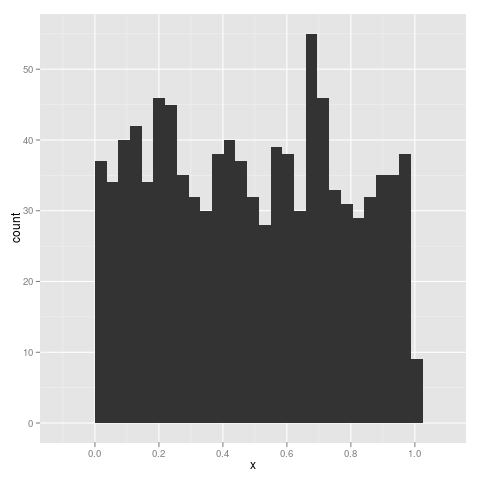
\includegraphics[scale=1]{./plots/hist.png}
  \caption{Here is a figure}
  \label{fig:hist}
\end{figure}


\section{Hello World!}


\bibliographystyle{aer}
\bibliography{paper.bib}

\end{document} 

